\section{Populationen}\label{populations}

% http://www.geatbx.com/docu/options-01.html

Unter einer Population versteht man eine Menge von Individuen. In diesem Kapitel
werden die Parameter beschrieben und untersucht, welche das Verhalten einer
einzelnen Population beziehungsweise mehrerer Populationen untereinander regeln.

\paragraph{Populationsgröße} Die Option \emph{NumberIndividuals} definiert die Anzahl der Individuen
pro Population. Genau genommen, ist hier die Anzahl pro Unterpopulation
(subpopulation) gemeint. Sollten mehrere Unterpopulationen verwendet werden,
exisitiert im Gesamten ein Mehrfaches der Populationsgröße an Individuen.
Der folgende Code-Ausschnitt enthält den Aufruf der {\tt testTsp()}-Funktion um
Populationsgrößen von 10 bis 1500 Individuen zu untersuchen.

\lstinputlisting[language=Matlab, firstline=6, lastline=7]{Code/suite.m}

\input{Chapters/gen/NumberIndividuals}

\noindent Die Ergebnisse zu den diversen Populationsgrößen sind in Tabelle
\ref{NumberIndividuals} präsentiert. Mit zunehmender Populationsgröße werden die
Wegkosten im Mittelwert kleiner und damit die Ergebnisse besser.
Die Standardabweichung wird ebenfalls kleiner, was bedeutet, dass die Ergebnisse
nicht mehr so weit um den Mittelwert schwanken. Allerdings steigt die Laufzeit
des evolutionären Algorithmus mit der Populationsgröße in etwa linear an,
weswegen man einen Kompromiss aus minimalen Wegkosten und der Laufzeit wählen
muss.

\begin{figure}[h!]
  \centering
  \includegraphics[width=1.0\textwidth]{Figures/gen/NumberIndividuals.png}
  \caption{Populationsgröße}\label{fig.numberindividuals}
\end{figure}

Um dies zu vereinfachen, sind in Abbildung \ref{fig.numberindividuals} die
mittleren Wegkosten und die Laufzeit dargestellt. Es ist ersichtlich, dass die
Kosten in Form einer Hyperbel abnehmen, bei kleinen Populationen ändern sie sich
noch sehr stark, je größer die Population wird, desto weniger verkürzt sich der
gefundene Weg. Als "'optimalen"' Wert für die endgültige Parametrisierung bietet
sich eine Größe von 100 Individuen an, da dort die Kosten-Kurve ihre größte
Krümmung aufweist und auch die Laufzeit noch in einem erträglichen Maße bleibt.


\paragraph{Unterpopulationen und deren Anzahl} Die Population aller Individuen
lässt sich wie oben beschrieben auf mehrere Unterpopulationen aufteilen.
Wird nur eine Unterpopulation spezifiziert, wird die gesamte Population als
eine panmiktische Population betrachtet. Werden hingegen mehrere Unterpopulationen
verwendet, entspricht dies bildlich mehreren Indianerstämmen, welche nebeneinander
existieren, aber sich auch hin und wieder Individuen stammesübergreifend paaren.
Diese stammesübergreifende Kombination wird bei den evolutionären Algorithmen
mit dem Begriff der Migration bezeichnet.

\input{Chapters/gen/NumberSubpopulation}

\begin{figure}[h!]
  \centering
  \includegraphics[width=1.0\textwidth]{Figures/gen/NumberSubpopulation.png}
  \caption{Unterpopulationen}\label{fig.numbersubpopulation}
\end{figure}

Die Tabelle \ref{NumberSubpopulation} stellt die Ergebnisse zu dem Parameter
\emph{NumberSubpopulation} bis hin zu einer Anzahl von 50 Unterpopulationen dar.
Wiederum werden die Ergebnisse mit zunehmender Anzahl besser, wobei auch
die Laufzeit wieder stark ansteigt, so dass statt einem optimalen Wert erneut
ein Kompromiss gefunden werden muss.
Wie in Abbildung \ref{fig.numbersubpopulation} ersichtlich, verläuft die
Kosten-Kurve in ähnlicher Form zu derjenigen der Populationsgröße. Um die
Laufzeit relativ gering zu halten, entscheiden wir uns für die weiteren Tests
und die optimale Konfiguration für eine Anzahl von 5 Unterpopulationen, womit
sich eine Gesamtpopulation von 500 Individuen ergibt.


\paragraph{Migration} Die Migrationsparameter beeinflussen die Art und Weise,
wie die verschiedenen Unterpopulationen gegenseitig ihre Genome austauschen.
Die Möglichkeit die Migration komplett zu deaktivieren, wurde nicht explizit
getestet, da dies vom Verhalten her identisch zu mehreren Läufen mit einer
einzigen Unterpopulation ist.

% http://www.geatbx.com/docu/options-05.html

Mit der Option \emph{Migration.Interval} lässt sich angeben, nach der wievielten
Generation jeweils eine Migration durchgeführt werden soll. Je kleiner der Wert,
desto häufiger werden die verschiedenen Stämme kombiniert. Die Tabelle
\ref{Migration.Interval} enthält die Ergebnisse zu den folgenden Tests:

\lstinputlisting[language=Matlab, firstline=16, lastline=18]{Code/suite.m}
\input{Chapters/gen/Migration.Interval}

\noindent Die besten Ergebnisse erhält man, wenn bei jeder Generation eine
Migration durchgeführt wird. Da dies auch keine negativen Auswirkungen wie
beispielsweise eine ansteigende Laufzeit aufweist, wird ein Wert von 1 für die
endgültige Parametrisierung gewählt.


Die Migrationsrate (Migration.Rate) definiert den Anteil jeder Population, welcher
während einer Migration modifiziert wird. Der Wertebereich reicht von 0 bis 1,
ein Wert von 0.2 bedeutet, das 20\% jeder Unterpopulation in den Migrationstopf
exportiert werden und gleich viele Individuen daraus wieder importiert werden.

\input{Chapters/gen/Migration.Rate}
\begin{figure}[h!]
  \centering
  \includegraphics[width=1.0\textwidth]{Figures/gen/Migration.Rate.png}
  \caption{Migrationsrate}\label{fig.migrationrate}
\end{figure}

\noindent Tabelle \ref{Migration.Rate} enthält die Ergebnisse zu den Testläufen.
Um eine bessere Übersicht über die verschiedenen Mittelwerte zu erhalten, sind
diese in Abbildung \ref{fig.migrationrate} dargestellt. Der "'optimale"' Wert
ist das Minimum der Kosten bei der Migrationsrate von 0.25.


Als weitere Option steht \emph{Migration.Topology} mit den folgenden 3 Verfahren
zur Verfügung, welche im Kapitel 8.3 \emph{Regional model - Migration} in
\citep{geatbx-ea} genauer beschrieben sind:
\begin{enumerate}
\setcounter{enumi}{-1} % begin first item with 0
\item \emph{complete net structure} - unbeschränkte Migration, jede
      Unterpopulation kann ihre Genome an alle anderen migrieren (siehe Abbildung
      \ref{fig.migrationtopology} a).
\item \emph{1-D neighborhood structure} - die Migration findet nur zwischen den
      nächsten Nachbarn statt. Unterpopulation 2 kann beispielsweise mit den
      Unterpopulationen 1 und 3 Genome austauschen.
\item \emph{1-D ring structure} - ähnlich zur Nachbarschafts-Struktur, allerdings
      werden die Genome nur zum nachfolgenden Nachbar weitergegeben (siehe Abbildung
      \ref{fig.migrationtopology} b).
\end{enumerate}

\begin{figure}[!h] \centering
    \subfigure[complete net structure]{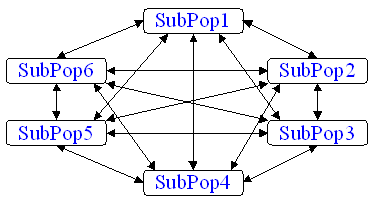
\includegraphics[width=0.49\textwidth]{Figures/migration-0.png}}\hfill
    \subfigure[1-D ring structur]{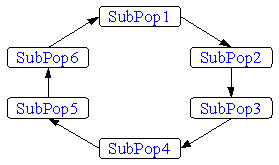
\includegraphics[width=0.45\textwidth]{Figures/migration-2.png}}
    \caption{Migrations-Topologien \citep{geatbx-ea}}
    \label{fig.migrationtopology}
\end{figure}

\input{Chapters/gen/Migration.Topology}

\noindent Die Tabelle \ref{Migration.Topology} stellt die Testergebnisse der
verschiedenen Topologieverfahren dar. Für die optimale Konfiguration bietet sich
\emph{1-D neighborhood structure} aufgrund des kleinsten Mittelwerts an, wobei
die anderen beiden Verfahren nur wenig schlechter abschneiden.


Der Parameter \emph{Migration.Selection} spezifiziert, wie die Individuen für
die Migration ausgewählt werden. Das \emph{GEATbx}-Framework bietet hierfür zwei
Möglichkeiten: ein Wert von 0 bedeutet, dass die Individuen zufällig ausgewählt
werden, wohingegen bei einem Wert von 1 die jeweils besten Individuen in den
Migrationstopf exportiert werden.

\input{Chapters/gen/Migration.Selection}

\noindent Die beiden Verfahren performen in etwa gleich gut, wie in Tabelle
\ref{Migration.Selection} ersichtlich ist. Aufgrund des etwas geringeren
Mittelwerts entscheiden wir uns für das Verfahren, bei dem die besten Individuen
ausgewählt werden (Parameterwert 1).

